%------------------------------------------------------------------------------%
% bachelor thesis															   %
% create by: Mario Preishuber												   %
% create date: 2014, Jan 01.												   %
%------------------------------------------------------------------------------%

\section{Analysis Tools} \label{sec:analysis_tools}

\subsection{Simple, artificial mutator}

We started our research with some simple, artificial mutators. Our aim was to get an overview of the behavior of different \JS garbage collectors. Therefore, we used three different mutators, which
\begin{itemize}
	\item Only allocate short-living objects,
	\item Only allocate long-living objects, and 
	\item A combination of the two above.
\end{itemize}
With these three mutators we started our measurements. We differ between so-called \textit{blackbox} and \textit{whitebox} data. The \textit{blackbox} data cover the execution time of a mutator and the real memory (resident set size) used of a mutator process. The \textit{whitebox} data require information about the \JS virtual machine. We get the \textit{whitebox} information from Google's V8. This data contains information about heap size, garbage collector frequency, and amount of memory that is collected (in byte).

\
Figure \ref{fig:mutator_keep_all_obj} presents measures of such a simple mutator. This mutator only allocates objects and keeps them live until the mutator terminates. The y-axis on the left shows the memory in MB and is used for the heap size (heap), resident set size (rss), and mark and sweep (mark-sweep). The y-axis on the right shows the number of live objects in thousands and on the x-axis the real time is displayed. Live objects are objects that are not collected by the garbage collector yet. For the live objects we expect a linear growing, but the Figure shows that the allocation of objects sometimes pauses which is a result of garbage collection. If we look at the resident set size and the heap size we see the dependency between these. The heap size presents more details about the garbage collection. The little spikes represent the collection of short-living objects. In our case this behavior shows a collection of system objects, because the mutator does not deallocate any objects. The bigger negative going flanks represent a mark and sweep phase of the garbage collector. A mark and sweep phase shows the collection of long-living objects. This simple mutator allows us to show some of the characteristics of a garbage collector.

\begin{figure}
	\centering
	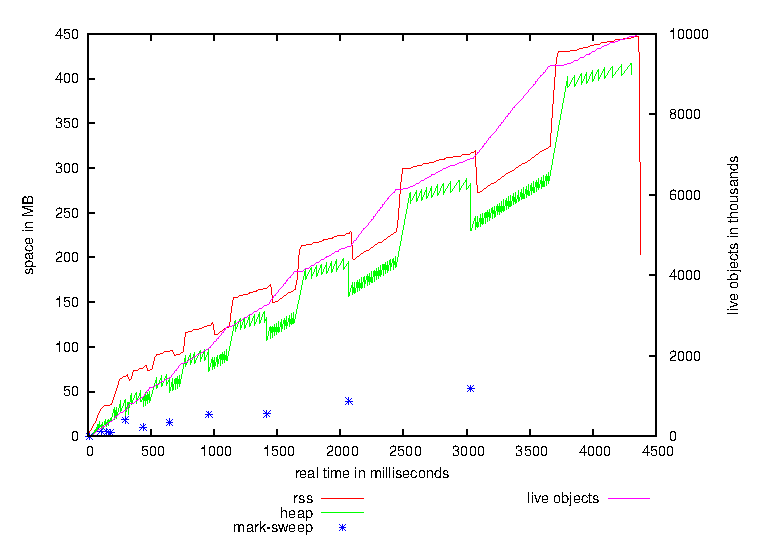
\includegraphics[width=0.5\textwidth]{keep_all_obj_rss_heap_mas_obj_time}
	\caption{Simple mutator which only allocates objects and never deallocates.}
	\label{fig:mutator_keep_all_obj}
\end{figure}

\
Figure \ref{fig:acdc_multi_exec_time} presents the execution time of a mutator which frequently deallocates a static amount of memory. We increase the lifetime of the allocated objects and measure the execution time. The lifetime is the duration since a object is allocated until it is deallocated. The so-called liveness of a object is similar to the lifetime. The x-axis of the figure shows the maximum liveness of the allocated objects and on the y-axis the execution time is displayed. A comparison of Google's V8 with Mozilla's \SM shows significant differences. If we look at the line of V8 we see some big spikes at a liveness of 30, 60, and 90. A reason for these spikes is the communication with the operating system. If the heap size of V8 overruns one of the internal bounds the process requests more memory from the operating system. If the heap size falls below such a bound the process responses memory to the operating system. In our case the heap size is toggling around such bounds. As a result there is a lot more communication with the operation system than usually which has a large impact on the execution time of the mutator.

\
The conclusion of our first mutator measurements is, that we are able to visualize characteristics of a garbage collector. Furthermore, we can show differences between different virtual machines. These mutators represent some corner cases, and if we think of a realistic \JS application there will be a different behavior.

\begin{figure}
	\centering
	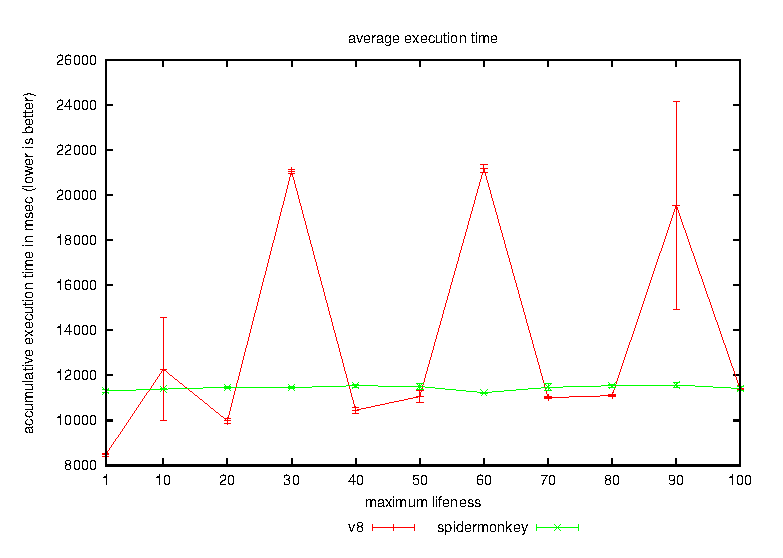
\includegraphics[width=0.5\textwidth]{acdc_multi_exec_time}
	\caption{Execution time: V8 vs. SpiderMonkey}
	\label{fig:acdc_multi_exec_time}
\end{figure}


%%%%%%%%%%%%%%%%%%%%%%%%%%%%%%%%%%%%%%%%%%%%%%%%%%%%%%%%%%%%%%%%%%%%%%%%%%%%%%%%
%%%%%%%%%%%%%%%%%%%%%%%%%%%%%%%%%%%%%%%%%%%%%%%%%%%%%%%%%%%%%%%%%%%%%%%%%%%%%%%%
%%%%%%%%%%%%%%%%%%%%%%%%%%%%%%%%%%%%%%%%%%%%%%%%%%%%%%%%%%%%%%%%%%%%%%%%%%%%%%%%

\subsection{Tools for obtaining a realistic heap model}

Developing a benchmark which is able to simulate a realistic \JS heap requires understanding the heap of real-world applications. As shown by some related work~\cite{JSMeter2009,JSMeter2010,Richards2011} the state-of-the-art benchmarks do not represent realistic heap behavior. In this section we describe our analysis to obtain a realistic heap model.

Our analysis are based on frequent generated snapshots of the \JS heap of a real-world application. The list of analyzed applications and proceeded user interactions is shown in Table \ref{tab:real_world_apps} on page \pageref{tab:real_world_apps}.
Figure \ref{fig:heap_structure_analysis} presents the complete toolchain we used to generate and analyze these snapshots. 

For the simulation of a realistic user interaction on a real-world application we used Selenium \cite{Selenium}. All user interactions we analyze are collected in the so-called \texttt{AutomatedUserInteraction} tool (see Section \ref{sec:automated_user_interaction}). For execution of a interaction we use a custom version of Chromium. We add a mechanism that periodic produces a snapshot of the \JS heap (for details see Section \ref{sec:custom_chromium}). 
The so-called \texttt{HeapSnapshotAnalyzer} analyzes these snapshots. The exact process is explained in Section \ref{sec:heap_snapshot_analyzer}.

\begin{figure}
	\centering
	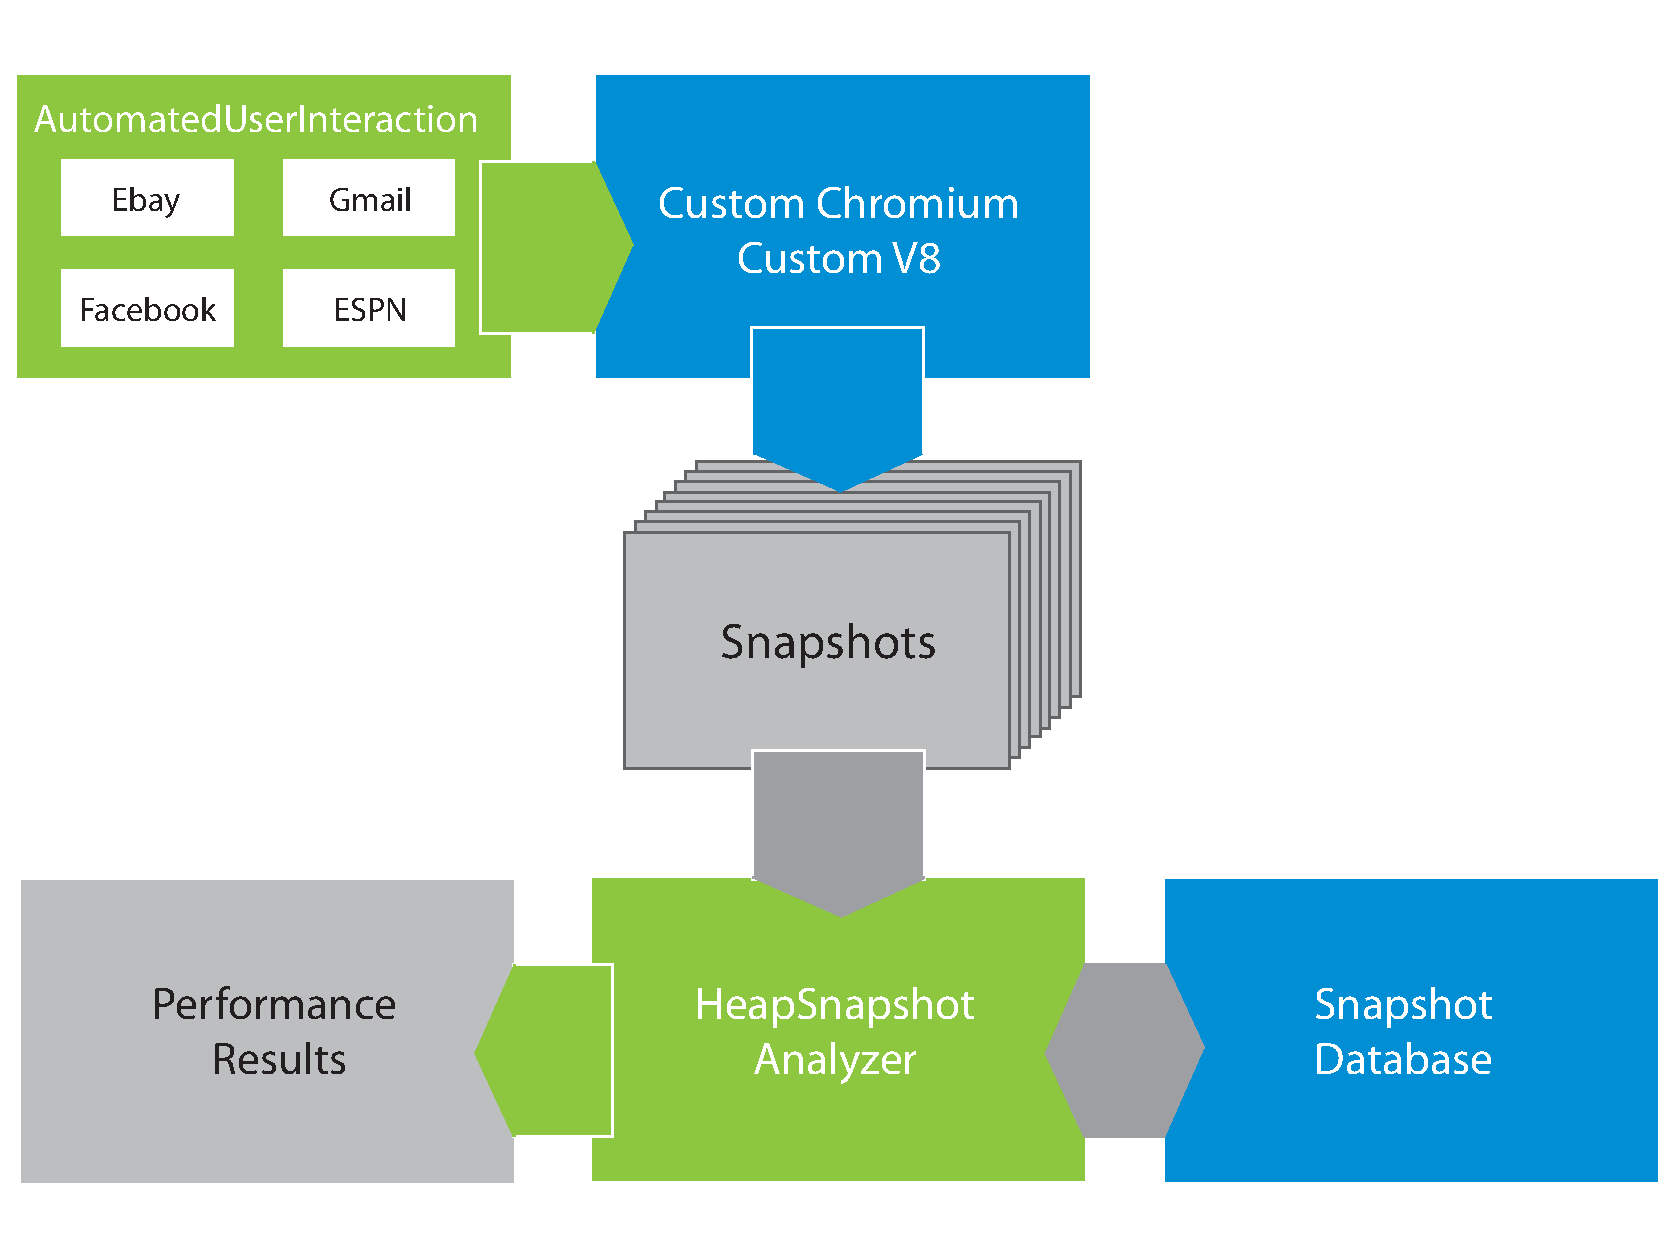
\includegraphics[width=0.5\textwidth]{solution_h}
	\caption{Tool chain for analyzing the JavaScript heap of a real-world web application}
	\label{fig:heap_structure_analysis}
\end{figure}


%%%%%%%%%%%%%%%%%%%%%%%%%%%%%%%%%%%%%%%%%%%%%%%%%%%%%%%%%%%%%%%%%%%%%%%%%%%%%%%%
%%%%%%%%%%%%%%%%%%%%%%%%%%%%%%%%%%%%%%%%%%%%%%%%%%%%%%%%%%%%%%%%%%%%%%%%%%%%%%%%
%%%%%%%%%%%%%%%%%%%%%%%%%%%%%%%%%%%%%%%%%%%%%%%%%%%%%%%%%%%%%%%%%%%%%%%%%%%%%%%%
	
\subsubsection{Tool for automating user interaction} \label{sec:automated_user_interaction}
To simulate a realistic user interaction we decided to automate this process by using Selenium \cite{Selenium}. A benefit of using Selenium is that we are able to repeat a user interaction as often as we want in exact the same way. Selenium also enables the opportunity to use different browsers. This feature allows us to run a user interaction on different browsers or use our own browser binary in a very easy way. For the heap snapshot generation we use our own custom Chromium binary (for details see Section \ref{sec:custom_chromium}). The Table \ref{tab:real_world_apps} shows all these real-world applications and the user interaction we perform. For each kind of web application the user interaction is tailored individually. The collection of all user interactions and a mechanism to switch between different browser binaries is provided by the so-called \texttt{AutomatedUserInteraction} tool.

\begin{table}
	\small
	\centering
	\begin{tabular}{l l}
		\toprule
		\textbf{Site} & \textbf{User interaction} \\ \midrule

		CNN 					& Read start page news, switch to category \textit{Europe}, 			\\ 
		\url{cnn.com} 			& read first article of \textit{Top Europe Stories}. 					\\ \midrule

		The Economist 			& Read start page news, switch to category 								\\ 
		\url{economist.com}		& \textit{Science \& technology}, read first article. 					\\ \midrule

		ESPN 					& Read start page news, switch to \textit{NASCAR}, 		 				\\ 
		\url{espn.com} 			& click on \textit{Results} and read site. 								\\ \midrule

		Hotmail 				& Sign in, check in-box, send email, read an email,						\\ 
		\url{hotmail.com} 		& delete it, and sign out. 												\\ \midrule

		Gmail 					& Sign in, check in-box, send email, read an email, 						\\ 
		\url{www.gmail.com} 	& delete it, and sign out. 												\\ \midrule

		Bing Search 			& Search for \textit{New York} and look at 								\\ 
		\url{bing.com} 			& resulting images and news. 											\\ \midrule

		Google Search 			& Search for \textit{New York} and look at 								\\ 
		\url{google.com}		& resulting images and news. 											\\ \midrule

		Facebook 				& Login and post a message. 											\\ 
		\url{facebook.com} 		&  																		\\ \midrule

		Google+ 				& Login and post a message. 											\\ 
		\url{plus.google.com} 	& 																		\\ \midrule

		Bing Maps 				& Search for directions from \textit{Austin} to \textit{Houston}		\\ 
		\url{maps.bing.com} 	& by car and walk. 														\\ \midrule

		Google Maps				& Search for directions from \textit{Austin} to \textit{Houston}		\\ 
		\url{maps.google.com} 	& by car and walk. 														\\ \midrule

		amazon 					& Search for the book \textit{Quantitative Computer Architecture},		\\ 
		\url{amazon.com} 		& add to shopping cart, look at cart. 									\\ \midrule

		eBay 					& Search for the book \textit{Quantitative Computer Architecture}. 		\\ 
		\url{www.ebay.co.uk} 	& 																		\\ \bottomrule

	\end{tabular}
	\caption{User interactions performed for the heap analysis of real web applications.}
	\label{tab:real_world_apps}
\end{table}

%%%%%%%%%%%%%%%%%%%%%%%%%%%%%%%%%%%%%%%%%%%%%%%%%%%%%%%%%%%%%%%%%%%%%%%%%%%%%%%%
%%%%%%%%%%%%%%%%%%%%%%%%%%%%%%%%%%%%%%%%%%%%%%%%%%%%%%%%%%%%%%%%%%%%%%%%%%%%%%%%
%%%%%%%%%%%%%%%%%%%%%%%%%%%%%%%%%%%%%%%%%%%%%%%%%%%%%%%%%%%%%%%%%%%%%%%%%%%%%%%%

\subsubsection{Custom Chromium} \label{sec:custom_chromium}
Obtaining a realistic \JS heap model requires information about objects and structure of a heap of a real-world \JS application. As explained in \cite{JSMeter2009} modifying the \JS engine of a browser is a good opportunity to get accurate information about the \JS heap. We use Chromium \cite{Chromium} the open source project of Google Chrome \cite{Chrome} to capture information about the \JS heap.

The Google DevTools \cite{DevTools} provide a functionality to generate heap snapshots. The problem is, there is no opportunity to periodic generate such a heap snapshot. We extend the V8 and implement such a mechanism that also stores the generated snapshots at a given directory. This mechanism works by using the Google V8 API function \texttt{TakeHeapSnapshot}. These snapshots contain some meta information, a nodes array, an edges array and a strings array. The nodes array and edges array represent a directed graph, the heap. The strings array is referenced by the nodes and edges array and contains only names. The complete list of properties of a node in the nodes array is shown in Table \ref{tap:heap_snapshot_node_fields} and the properties of the edges are shown in Table \ref{tap:heap_snapshot_edge_fields}. To control the generation of heap snapshots, we extend the V8 with following flags:
\begin{itemize}
	\item \texttt{automatic heap snapshots}
	\item \texttt{heap snapshot interval}
	\item \texttt{heap snapshot prefix} 
\end{itemize}	
The \texttt{automatic heap snapshots} flag enables the generation of snapshots in general, default it is \texttt{false}. To control how frequent snapshots are generated the \texttt{heap snapshot interval} flag is used, default value is 64KB. Every time \texttt{n} KB are allocated a snapshot is taken. The third flag, \texttt{heap snapshot prefix}, is only a prefix of the generated snapshot files, default value is \textit{snapshot}. The produced snapshots are numbered consecutively until the \texttt{automatic heap snapshots} flag is set to \texttt{false} or the mutator terminates. The extension of such files is \textit{.heapsnapshot}. 

%%%%%%%%%%%%%%%%%%%%%%%%%%%%%%%%%%%%%%%%%%%%%%%%%%%%%%%%%%%%%%%%%%%%%%%%%%%%%%%%
%%%%%%%%%%%%%%%%%%%%%%%%%%%%%%%%%%%%%%%%%%%%%%%%%%%%%%%%%%%%%%%%%%%%%%%%%%%%%%%%
%%%%%%%%%%%%%%%%%%%%%%%%%%%%%%%%%%%%%%%%%%%%%%%%%%%%%%%%%%%%%%%%%%%%%%%%%%%%%%%%

\subsubsection{Tool for analyzing heap snapshots} \label{sec:heap_snapshot_analyzer}
The steps before describe how we capture data about a realistic \JS heap. Now we want to explain how we analyze the generated snapshots. 

For each real-world application, listed in Table \ref{tab:real_world_apps}, we use a sample rate of 4KB, i.e., a snapshot is created whenever 4KB of new objects are allocated by the application. The number of generated snapshots depends on the amount of memory which is allocated by a real-world application and the runtime of a user interaction. When a heap snapshot is taken the garbage collector is automatically called. As a result a snapshot only contains live objects. 

However, we use a PostgreSQL \cite{PSQL} database, version 9.3, to analyze the snapshots. To handle the preparation of a snapshot for the database as well as the analysis we develop a tool. This tool is a Java application that we call \texttt{HeapSnapshotAnalyzer}. For a realistic heap model, we are interested in the distribution of object types, sizes and lifetimes, the number of out-going edges, and the distance from a GC root to a object. A heap snapshot represents all live objects of the \JS heap and each object has a type. The complete list of object types is shown by Table \ref{tap:heap_snapshot_node_types}. An object also has a size, which represents the amount of byte the object needs on the heap. The number of outgoing edges represents the number of references an object holds. A snapshot contains special nodes of type synthetic which represent GC roots. These nodes has are used to compute the root distance. The root distance represents the minimum number of edges to reach a node from a GC root. How we compute these properties is described in Section \ref{sec:analysis_mutator}.